\section{Equilibrio y cinética}

\subsection*{Constantes de equilibrio}

La constante de equilibrio $K_C$ es de una reacción con rendimiento menor a 100\%. $[A]$ se refiere a la concentración molar de $A$ (molaridad):
$$\ce{
aA + bB \rightleftharpoons cC + dD
}$$
$$
K_C = \dfrac{[C]^c \cdot [D]^d}{[A]^a\cdot [B]^b}
$$

La constante de equilibrio $K_P$ es para gases. $(P_A)$ es la presión parcial de $A$.
$$
K_P = \dfrac{(P_C)^c \cdot (P_D)^d}{(P_A)^a \cdot (P_B)^b}
$$


\subsubsection*{Relación con ácidos y bases}

\hfil$K_a \cdot K_b = K_w = 10^{-14}$\hfil

$$\text{p}K_a + \text{p}K_b = \text{p}K_w = 14$$


\subsection*{Reacciones}

Una reacción endotérmica es aquella que consume calor. Una exotérmica lo libera.

\subsubsection*{Principio de Le Chatelier}

``Cuando se perturba un sistema en equilibrio, el mismo sistema va volver a tener al equilibrio.''

Una reacción \textbf{endotérmica} (consume calor), tenderá hacia los productos cuando aumente la temperatura.

Una reacción \textbf{exotérmica} (libera calor), tenderá hacia los productos cuando disminuya la temperatura.

Al aumentar la presión de un sistema gaseoso, el equilibrio tenderá al lado que disminuya la presión.

\begin{figure}[H]
    \centering
    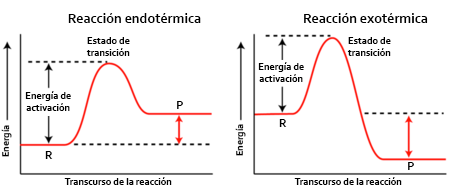
\includegraphics[width=0.8\textwidth]{Images/energia-activacion.png}
\end{figure}
